\section{Principes de DICOM}

	\subsection{Objectifs de DICOM}
	
	\frame
	{
		\frametitle{Buts g\'en\'eraux}
		\begin{itemize}
			\item<1-> Trouver un langage commun pour l'\'echange (images et donn\'ees pertinentes) entre \'equipements d'imagerie : mettre en place un standard.
			\item<2-> Pousser les vendeurs \`a parler et comprendre ce langage commun.
			\item<3-> Standardiser :
			\begin{itemize}
				\item<4-> le stockage (i.e. format de fichier) ;
				\item<5-> et la communication des donn\'es (i.e. protocoles de communication).
			\end{itemize}
		\end{itemize}
	}
	
	\frame
	{
		\frametitle{Buts sp\'ecifiques}
		
		Il faut que lors de l'installation d'une nouvelle modalit\'e, le DICOM permette, sans changement d'un quelconque composant logiciel (\emph{i.e. Plug \& Play} :
		\begin{itemize}
			\item<1-> l'interrogation du PACS ;
			\item<2-> la r\'ecup\'eration des images cr\'e\'ees par d'autres syst\`emes ;
			\item<3-> l'affichage des images ;
			\item<4-> et la production d'images lisibles par les syst\`emes d'autres constructeurs.
		\end{itemize}
	}

	\subsection{Fondements th\'eoriques}

	\frame
	{
		\frametitle{Prescription d'un examen radiologique}
		\begin{itemize}
			\item Sch\'ematisation de la proc\'edure :
			%\includegraphics<2->[width=\linewidth]{./figures/scenario-1.png}
			%\includegraphics<3->[width=\linewidth]{./figures/scenario-2.png}
			%\includegraphics<4->[width=\linewidth]{./figures/scenario-3.png}
			%\includegraphics<5->[width=\linewidth]{./figures/scenario-4.png}
			%\includegraphics<6->[width=\linewidth]{./figures/scenario-5.png}
			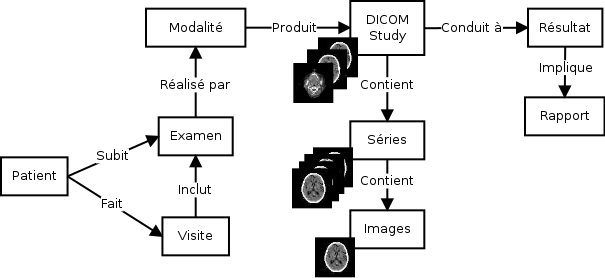
\includegraphics[width=\linewidth]{./figures/scenario.png}
			\item<2-> DICOM d\'ecrit ces donn\'ees et ces relations.
			\item<3-> La pr\'ecision du contenu et des liens d\'epend des outils et des utilisateurs (\emph{e.g.} RIS, PACS).
		\end{itemize}
	}

	\frame
	{
		\frametitle{Traduire le r\'eel en num\'erique}
		
		\begin{itemize}
			\item Un objet DICOM combine donc :
			\begin{itemize}
				\item<2-> des donn\'ees, ou informations (e.g. nom du patient, donn\'ees de l'image,\ldots) ;
				\item<3-> et services, ou fonctions (e.g. sauvegarder, imprimer,\ldots).
			\end{itemize}
			
			\item<4-> Le traitement DICOM d'une information consiste alors \`a regrouper :
			\begin{itemize}
				\item<5-> les donn\'ees, contenues dans un \emph{Information Objet}, que le standard d\'efinit gr\^ace \`a une \emph{Information Object Definition} (ou \emph{IOD}) ;
				\item<6-> et une fonction sp\'ecifique, ou \emph{Service}, d\'efinie par un \emph{DICOM Message Service Element} (ou \emph{DIMSE}).
			\end{itemize}
		\end{itemize}
	}
	
	\frame
	{
		\frametitle{SOP Class UID}

		\begin{itemize}
			\item La combinaison Information Objet + Service est :
			\begin{itemize}
				\item<2-> appel\'ee \emph{Service/Object Pair} (ou \emph{SOP}) ;
				\item<3-> un \'el\'ement important pour d\'eterminer la conformit\'e au standard ;
				\item<4-> identifi\'ee par un identifiant unique nomm\'e \emph{SOP Class UID}.
			\end{itemize}
		
			\item<5-> Standard DICOM = annuaire de SOP.\\
			SOP Class UID = num\'ero unique pour trouver \`a quelle paire Service/Objet correspond un objet DICOM.
			\item<6-> Analogie : annuaire\\
			Une entr\'ee = paire \{t\'el\'ephone $+$ adresse\}.
			\item<7-> Exemples de SOP Class UID :
			\begin{description}
				\item<8->[$1.2.840.10008.5.1.4.1.1.1$] CR Image Store (enregistrer un CR) ;
				\item<9->[$1.2.840.10008.5.1.4.1.1.2$] CT Image Store (enregistrer un CT).
			\end{description}
		\end{itemize}
	}
	
	\frame
	{
		\frametitle{Sch\'ema de construction du SOP}
		\begin{center}
			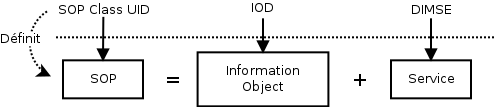
\includegraphics[width=\linewidth]{./figures/sop-definition.png}
		\end{center}		
	}

